\documentclass[a4paper]{article}
\usepackage[a4paper]{geometry}
\usepackage{listings}
\usepackage{textcomp}
\usepackage{color}
\usepackage{graphicx}
\graphicspath{ {images/} }

\definecolor{dkgreen}{rgb}{0,0.6,0}
\definecolor{gray}{rgb}{0.5,0.5,0.5}
\definecolor{mauve}{rgb}{0.58,0,0.82}

\lstset{frame=tb,
  language=Java,
  aboveskip=3mm,
  belowskip=3mm,
  showstringspaces=false,
  columns=flexible,
  basicstyle={\small\ttfamily},
  numbers=none,
  numberstyle=\tiny\color{gray},
  keywordstyle=\color{blue},
  commentstyle=\color{dkgreen},
  stringstyle=\color{mauve},
  breaklines=true,
  breakatwhitespace=true,
  tabsize=3
}
\begin{document}
\section{Coordinates}

\paragraph{}
Our basic unit for positioning is a Coordinate which is a two dimension cartesian coordinate system location denoted by X and Y positions, for the former an horizontal point in the x axis and for the latter a vertical point in the y axis, This class is used within the whole system in many other clases like the and lane for the start points and end points. It is also used for the intersection and vehicle position.

\paragraph{}
The most important features for the Coordinate class besides the getters and setters for the x and y positions are the overloading of the equal operator to enable Coordinate comparisons, addition and subtraction methods and the capability to add a step to a position regarding the cardinal direction.

\begin{lstlisting}

//Adds a step to the coordinate based on map direction
public Coordinate addStep(MapDirection mapDirection) {
        Coordinate sum = new Coordinate(-1,-1);

        switch (mapDirection) {
            case NORTH:
                sum.setY(this.getY() - 1);
                sum.setX(this.getX());
                break;
            case SOUTH:
                sum.setY(this.getY() + 1);
                sum.setX(this.getX());
                break;
            case EAST:
                sum.setX(this.getX() + 1);
                sum.setY(this.getY());
                break;
            case WEST:
                sum.setX(this.getX() - 1);
                sum.setY(this.getY());
                break;
        }

        return sum;
    }
\end{lstlisting}

\section{Components}
\paragraph{}
We have defined a common denominator between objects that we are able to add to a map.
Currently we have two types of components:

\begin{itemize}  
\item Roads
\item Intersections
\end{itemize}

\paragraph{}
The lanes are embedded in roads and vehicles are objects that work on top of a map. The same for traffic lights that work on top of an intersection. Like the Coordinate, the components are used widely in the whole system.

\paragraph{}
To use components we capture the object and cast it to an instance of either a Road or an Intersection depending on the case we are able to interact with the component treating it as the former or the latter.

\begin{lstlisting}
//Snippet of how the method differentiates between different types of instances
if(component instanceof Intersection) 
    {
    	...
    }
    
    else if(component instanceof Road) 
    {
    	...        
    }
\end{lstlisting}

\section{Map}
\paragraph{}
It consists in a mixture of Roads and Intersections and it is the graph structure that our map holds. In this class there are substantial functions that allow us to communicate with the different components.  After accessing the Roads that reside in the map we can also access Lanes, Cells, etc. The Map class interacts with the MapGrid class by using a getter and setter to a valid MapGrid. In this class there are two important functions which give us the capability of loading and saving maps. For the latter it would save the serialised map object to the Map directory; for the former it would load a saved map model with its composite components.

\begin{lstlisting}
    public void saveMap(String fileName)
    {
        try
        {
            File directory = new File(MAP_DIR);
            if(!directory.exists()) directory.mkdir();
            
            String path = MAP_DIR + fileName;
            File file = new File(path);
            if(!file.exists()) file.createNewFile();
            // save the map
            FileOutputStream fileOut = new FileOutputStream(path);
            ObjectOutputStream out = new ObjectOutputStream(fileOut);
            out.writeObject(this);
            out.close();
            fileOut.close();
        }catch(IOException i)
        {
            i.printStackTrace();
        }
    }
\end{lstlisting}

\section{Map Grid}

\paragraph{}
The map grid is the underlying structure of our Map. It is a 2D Array of the class Components which has embedded a Road, Intersection or an Empty Cell. The map grid has a width and height which represents the size of the map. One of the most important functionalities is to add a Component to the grid which in this case adds an Intersection or a Road.

\begin{lstlisting}
//Adds a Component to the map grid structure
public boolean addComponent(Component c) 
    {
        if(c instanceof Intersection) {
            ...
        }
        else if(c instanceof Road) {
            ...
    	}
    }
\end{lstlisting}

\paragraph{}
We were able to test the model of our maps in a text-based fashion then subsequently when the relevant tests were passed, we were able to integrate it with a graphic user interface view.


\centerline{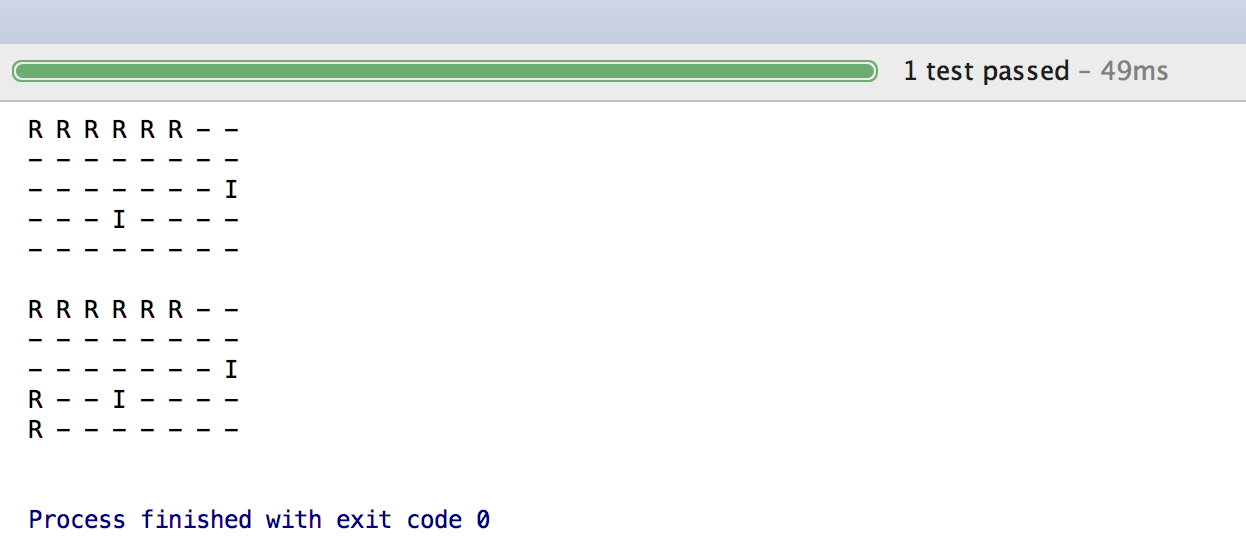
\includegraphics[scale=0.5]{test_mapgrid}}

\section{Road}

\paragraph{}
We have defined a road as a container for 0 or more lanes with a start point and an end point of type Coordinate. This allows us to track the position of the road and consequently add an Intersection or not to the end of the road. Each road is connected to at most 2 intersections. Our roads can be of size 1 to n and only can be drawn horizontally or vertically according to the start and end point locations. Our Simulation system has limited the number of lanes of a road to 2 with a left-hand traffic fashion. Another limitation is the size of the road which it\textsc{\char13}s minimum size is 1 and its maximum size is 30 . If we do not assign an intersection to any end of the road, the vehicle will leave the simulation after reaching the end.

\section{Lane}

\paragraph{}
A lane is part of a road where the vehicles actually move. The lane is divided in a certain amount of cells normally the minimum is 1 and the maximum is the difference between the start point and the end point. In our simulation the maximum is also 30. In a lane the cellular automata model takes place. Each lane is denoted as a queue with a length.

\paragraph{}

The lane also has start and end coordinates. Additional to the road attributes, it has a map direction which we designated as an ENUM with the values NORTH, SOUTH, EAST, WEST and ERROR. We didn\textsc{\char13}t compute the map direction because a lane can have a dimension of one cell which can imply either a horizontal direction or a vertical direction but not the specific cardinal direction. To create a lane we must consider 4 aspects regarding the cardinality:

\begin{itemize}
\item If the map direction is North, then the lane\textsc{\char13}s start point is the road\textsc{\char13}s start point and the lane\textsc{\char13}s end point is the road\textsc{\char13}s end point.
\item If the map direction is South, then the lane\textsc{\char13}s start point is the road\textsc{\char13}s end point and the lane\textsc{\char13}s end point is the road\textsc{\char13}s start point.
\item If the map direction is East,  then the lane\textsc{\char13}s start point is the road\textsc{\char13}s start point and the lane\textsc{\char13}s end point is the road\textsc{\char13}s end point.
\item If the map direction is West,  then the lane\textsc{\char13}s start point is the road\textsc{\char13}s end point and the lane\textsc{\char13}s end point is the road\textsc{\char13}s start point.
\end{itemize}

\begin{lstlisting}
	//Road creation with the MapExamples class
	Road r1 = new Road(new Coordinate(2,1), new Coordinate(2,1));
	Road r2 = new Road(new Coordinate(1,2), new Coordinate(1,2));
	Road r3 = new Road(new Coordinate(3,2), new Coordinate(3,2));
	Road r4 = new Road(new Coordinate(2,3), new Coordinate(2,3));
	
	r1.addLane(new Lane(r1.getStartLocation(),r1.getEndLocation(), MapDirection.EAST));
	r1.addLane(new Lane(r1.getEndLocation() ,r1.getStartLocation(), MapDirection.WEST));
	
	r2.addLane(new Lane(r2.getEndLocation(),r2.getStartLocation(), MapDirection.NORTH));
	r2.addLane(new Lane(r2.getStartLocation(),r2.getEndLocation(), MapDirection.SOUTH));
	
	r3.addLane(new Lane(r3.getEndLocation(),r3.getStartLocation(), MapDirection.NORTH));
	r3.addLane(new Lane(r3.getStartLocation(),r3.getEndLocation(), MapDirection.SOUTH));
	
	r4.addLane(new Lane(r4.getStartLocation(),r4.getEndLocation(), MapDirection.EAST));
	r4.addLane(new Lane(r4.getEndLocation(),r4.getStartLocation(), MapDirection.WEST));
\end{lstlisting}

\section{Graphical User Interface}

\subsection{Map component drawings}
\paragraph{}
For the map creation we are using a suite of Panes which are included in the JavaFX Software Platform. We use stacked panes which allow us to treat different panes like layers and that grants us major management. The whole grid layout consists on a GridPane which is a flexible grid of rows and columns that holds in each row and column a specific pane. Each pane is a box which can either be grass (Empty) a Road or an Intersection. The Road is a stack pane that has a rough grey background and the arrows of the lane are drawn programatically in each square. The intersection is  drawn with the same background as a Road but in addition it has a yellow diagonal cross. The traffic lights are also drawn programatically. All are drawings are of our own authorship because we have used the tool GIMP which is an open source graphic editor. It\textsc{\char13}s worth mentioning that the size of each stack pane is dynamic and we are able to fix the measure by changing the resizeFactor that is an important attribute used in many of our drawings. We are able to create grids of different sizes limited to an ample range from 5x5 to 30x30.
\subsection{Layout GUI}
\paragraph{}
The LayoutGUI class manages the drawings for the grass with a generic function that gets called by any map component drawing function. It draws the map component given a path to an image:
\begin{lstlisting}
/**
     * The generic function that gets called by any map component drawing function. It draws the map component given
     * a path to an image.
     * @param path the path to the image for this GUI square
     * @return the StackPane representing this GUI square, based on the provided image
     */
private StackPane drawLayout(String path) {
        Image image = new Image(path);

        Image im  = new Image(path,image.getWidth()*this.getResizeFactor().getResizeX(),
        image.getHeight()*this.getResizeFactor().getResizeY(),false,false);

        ImageView iv = new ImageView(im);

        StackPane stackPane = new StackPane();

        stackPane.getChildren().add(iv);

        return stackPane;
    }
\end{lstlisting}

\subsection{GUI Decorators}
\paragraph{}
Our implementation has considered the use of the Decorator Pattern to extend the functionalities of each component so that the objects can be drawn by wrapping the original object and invoking a draw method for each component. There are 5 main wrappers IntersectionDecorator, MapGridGUIDecorator RoadGUIDecorator, TrafficLightDecorator and VehicleDecorator.

\subsubsection{IntersectionDecorator}
\paragraph{}
Associates an Intersection GUI with an instance of an Intersection. Each has up to 4 TrafficLightDecorators that live inside this GUI. The Intersection does not have any explicit circles itself, it relies on the circles of each TrafficLightDecorator that is associated with each TrafficLight in the Intersection instance. Exactly one IntersectionDecorator is created for exactly one Intersection.

The most important functionality of the Intersection decorator is the drawIntersection method that draws the wrapped Intersection and produces a visual junction with traffic lights embodied in a stack pane.

\begin{lstlisting}
//Draws the intersection to display it in the GUI
public StackPane drawIntersection() 
{
	...
	return stackPane;
					
}
\end{lstlisting}

\subsubsection{RoadGUIDecorator}
\paragraph{}
This class defines how roads are drawn and displayed in the view. Each Road instance will have exactly one of these decorators associated with it.

\subsubsection{TrafficLightDecorator}
Traffic Light GUI Logic is implemented here. One instance of this class is associated with exactly one instance of a TrafficLight.

\subsubsection{VehicleGUIDecorator}
This class is used not only to draw vehicles but to display them in the graphic user interface and also animate the object along the lanes. Each vehicle will have exactly one VehicleGUIDecorator associated with it. We have defined different states of the vehicle so we can track their movements and make them move properly:

\begin{itemize}
\item state 0 is when a vehicle isn\textsc{\char13}t moving
\item state 1 means that the vehicle is moving straight.
\item state 2 means that the vehicle has entered an intersection
\item state 3 is a state where the vehicle has been deleted or has exited the simulation.
\end{itemize}

\subsection{Evolution of the vehicle drawing and animation}
\paragraph{}
After the grid was able to be drawn dynamically, the vehicle had to move on top of the lanes so at first it was challenging because there was a lack of documentation about animation between cells pertaining to a grid pane. The method used to overcome the problem was to read and try each attribute of the drawing until we were able to place the rectangle which represents a car in the correct position wether it was needed to be placed horizontally or vertically and also in the correct grid pane cell. The class function that draws the vehicle was initially coded to act like a big rectangle that would fill the entire cell of the lane and the class function moveVehicleGUI would add the movement according to the amount of steps we wished the object to travel. This initial approach was working correctly; however, we needed to integrate the whole movement with a Ticker which was still under construction and the behaviour was uncertain by the time it was finished due to its incompatibility with JavaFX.

\paragraph{}
We were able to overcome the integration with the Ticker and by that time, we decided that the steps of each movement were going to be one for an average behaviour and two for an aggressive behaviour. The vehicle was able to travel from a start point to the end of a lane with no problem. The next challenge was to animate the vehicle when it passed the intersection but this problem wasn\textsc{\char13}t so easy to solve. The drawing wasn\textsc{\char13}t showing were we wanted it to be place therefore it took more effort than expected to close the issue. Meanwhile other team members where working with the model and the car movement was in its turning phase which still had flaws because it didn\textsc{\char13}t turn properly. However, we were able to rotate the object with a nested rotate transition and finally the integration was successful. Currently the moveVehicleGUI method doesn\textsc{\char13}t use the step parameter anymore because it works directly with the coordinates that the model grants to the wrapper so it can animate properly.

\end{document}
